\documentclass[10pt, letter]{report}
\usepackage[utf8]{inputenc}
%\usepackage[frenchb]{babel}
\usepackage[T1]{fontenc}
%\usepackage{a4wide}
\usepackage{indentfirst}
\usepackage{amsfonts}
\usepackage{graphicx,graphics}
\usepackage{amssymb}
\usepackage{rotate}
%\usepackage{pgf,pgfarrows,pgfnodes,pgfautomata,pgfheaps,pgfshade}
\usepackage{multicol}
\usepackage{multirow}
\usepackage{epsf}
\usepackage{epsfig}
\usepackage{amsmath}
\usepackage{psfrag}
\usepackage{color}
%\usepackage{draftcopy}
\usepackage{NOMBRE}
%\usepackage{marvosym}
\usepackage{dcolumn}
\usepackage{subfigure}
\usepackage{color}
\usepackage{fancybox}
\usepackage{fancyhdr}
\usepackage{hyperref}
%\usepackage{xspace}
%\usepackage[breaklinks=true]{hyperref}
%\usepackage{transfig}
\usepackage{lastpage}
\usepackage{placeins}

\usepackage{caption}
\usepackage{smartdiagram}
\usepackage{booktabs}
\usepackage{float}
\restylefloat{table}

\usepackage{pstricks, pst-3d}

\pagestyle{headings}
%\usepackage{palatino}
\topmargin=-1cm
\rightmargin=0cm
\headheight=1cm
\headsep=1cm
\footskip=1cm
\textheight=21.5cm
\textwidth=16.4cm
\oddsidemargin=-0.5cm
\evensidemargin=-0.5cm
%\usepackage{braket}
%\newtheorem{theo}{Théorème}
%\bigskip
\def\Tiny{\fontsize{3pt}{3pt}\selectfont}



\newcolumntype{M}[1]{>{\raggedright}m{#1}}

\newcommand{\ket}[1]{\ensuremath{\left| #1 \right\rangle}}
\newcommand{\bra}[1]{\ensuremath{\left\langle #1 \right|}}
\newcommand{\vect}[1]{\ensuremath{\overrightarrow{#1}}}
\newcommand{\encadre}[1]{\begin{equation}
\begin{tabular}{|c|}
\hline
\\
$\displaystyle \; #1 \;$\\
\\ \hline
\end{tabular}
\end{equation}}


\newcommand{\encadredeux}[1]{\begin{equation}
\begin{tabular}{|c|}
\hline
\\
$\displaystyle \; #1 \;$\\
\\ \hline
\end{tabular}\nonumber
\end{equation}}


\newcommand{\encadrebut}[1]{\begin{equation}
\begin{tabular}{|c|}
\hline
\\
$\displaystyle \; \mbox{\underline{But} :  #1} \;$\\
\\ \hline
\end{tabular}\nonumber
\end{equation}}


\newcommand{\moy}[1]{\ensuremath{\left\langle #1 \right\rangle}}
\newcommand{\ave}[1]{\ensuremath{\bar{#1}}}



\title{Modélisation Silice}
\date{Juillet 2012}
\author{Jean-Yves DELANNOY}

\newcommand{\f}[2]{{\ensuremath{\mathchoice%
        {\dfrac{#1}{#2}}
        {\dfrac{#1}{#2}}
        {\frac{#1}{#2}}
        {\frac{#1}{#2}}
        }}}

%\bibliographystyle{plain}
%\bibliography{bibli.bib}


\renewcommand{\=}{\, =\, }
\newcommand{\+}{\, +\, }
\renewcommand{\-}{\, -\, }
\newcommand{\vv}{\vspace{-0.5cm}}

\newcommand{\trip}[3]{\ensuremath{\left[T_{#1},\left[T_{#2},T_{#3}\right]\right]}}

\newcommand{\eqn}[1]{\begin{equation} #1 \end{equation}}


\newcommand{\property}[2]{{\underline{Propriété #1}} : 
{\it \bf #2}
}

\newcommand{\ie}{{\it i.e. }}
\newcommand{\cf}{{\it cf.~}}

\newcommand{\bc}[1]{\begin{tabular}{|c|}
\hline
#1\\
\hline\end{tabular}_{p\times p}}

\newcommand{\entier}[1]{\left[\hspace{-1ex}\left[\hspace{0.5ex}#1\hspace{0.5ex} \right]\hspace{-1ex}\right]}





%%%%%%%%%%%%%%%%%%%%%%%%%%%%%%%%%%%%%%%%%%%%%%%%%%%%%%%%%%%%
% Show subsubsection numbers as a letter
\setcounter{secnumdepth}{3}
\makeatletter
\renewcommand\thesubsubsection{\thesubsection .\@alph \c@subsubsection}
\makeatother

%%%%%%%%%%%%%%%%%%%%%%%%%%%%%%%%%%%%%%%%%%%%%%%%%%%%%%%%%%%%
% make graph and figure scaling uniform

\newcommand{\setpath}[1]{
  \graphicspath{{figures/#1/}{graphes/#1/}}
}

\newcommand{\graphscale}{0.27}
\newcommand{\figscale}{0.6}

\newcommand{\includefigure}{\includegraphics}
\newcommand{\includegraph}{\includegraphics}

\newcommand{\includescaledgraph}[1]{%
  \includegraphics[scale=\graphscale]{#1}%
}

\newcommand{\includescaledfigure}[1]{%
  \includegraphics[scale=\figscale]{#1}%
}


\newlength{\espace}
\setlength{\espace}{0.8cm}
\setlength{\footskip}{1cm}
\definecolor{gris}{gray}{0.5}
%\graphicspath{{../}{C:/Users/jdelanno/Documents/Presentation/IMAGES/}{C:/Users/jdelanno/Documents/COMPNANOCOMP/Deliverables/}}


%\graphicspath
%\usepackage{fancyhdr}
\setlength{\headheight}{25pt}

 
\pagestyle{fancy}
%\renewcommand{\chaptermark}[1]{\markboth{#1}{}}
\renewcommand{\sectionmark}[1]{\markright{#1}{}}
\renewcommand{\headrulewidth}{0pt} % remove lines as well
\renewcommand{\footrulewidth}{0pt}

\fancyhf{}
\fancyfoot[LE,RO]{\thepage}
%\fancyfoot[RE]{\textit{\rightmark}}
%\fancyfoot[LO]{\textit{\rightmark}}
%\fancyfoot[RE,LO]{\textit{\rightmark}\\
%\vspace*{1.5cm}
%\textcolor{gris}{\Tiny Centre de Recherches et Technologies de Lyon : 85, rue des Frères Perret. BP 62. F-69192 Saint-Fons. Tél. : +33 4 72 89 67 89. Fax : +33 4 72 89 68 63\\
%Siret : 622 037 083 00285\\
%Dénomination sociale : Rhodia Opérations. 40, rue de la Haie Coq. 93306 Aubervilliers Cedex. France. Tél. : + 33 1 53 56 50 00. Fax : + 33 1 53 56 55 55\\
%Société par Actions Simplifiée au capital de 695 897 850 euros. RCS Bobigny 622 037 083. TVA intracommunautaire 41 622 038 083\\
%{\bf www.rhodia.com}}
%}

\fancyhead[LE,RO]{\hspace*{2cm}
\includegraphics[width=0.08\textwidth]{Logo_Solvay}}

\usepackage[final]{pdfpages}


\newcommand{\degre}{$^{\circ}\mathrm{C}\,$}


\begin{document}


\title{\textbf{COMPNANOCOMP Final Report.}}
%treatment


\author{P. J. Kowalczyk}
\date{\today}

\vspace*{1cm}
\hspace*{-1cm}\begin{tabular}{p{0.49\textwidth}p{0.08\textwidth}p{0.42\textwidth}}
{\bf Date:} \today & \multicolumn{2}{r}{{\huge \bf{Technical Report }}}\\
\\
\hline
\\
{\bf De} : Paul Kowalczyk  & \bf{\`A:} & Jean-Yves Delannoy \\
&& Alessio Tamburro \\

 \\
{\bf Copie} :   \\
{\bf Ref} :&  {\bf Pages : }  & \pageref{LastPage} \\
\\
\hline
\\
\multicolumn{3}{c}{\LARGE Machine Learning} \\
\\
\multicolumn{3}{c}{\LARGE Final Report.} \\
\\
\hline
\end{tabular}
%
\vspace*{2cm}

\begin{multicols}{2}
Informatics-based statistical learning approaches can be a promising alternative to quantum mechanical computations for calculating bandgaps. With this report we demonstrate a systematic feature-engineering approach and a robust learning framework for efficient and accurate predictions of electronic bandgaps of sulfides. The models developed are validated and tested using data science best practices. Following a feature-engineering protocol that included (1) removing features with zero variance, (2) removing highly correlated features, and (3) removing features that result from linear combinations of other features, six machine learning algorithms were tested. These algorithms were: multiple linear regression, partial least squares, support vector machines, k-nearest neighbors, boosted trees, and random forests. Models were built using each algorithm. A training set of 1593 sulfide band gap energies used for model construction was retrieved from the Materials Project. The predictive accuracy of each model was evaluated using a test set of 396 sulfide band gap energies, also retrieved from the Materials Project. Using the adjusted \( R^2 \) of the test set results, the boosted trees machine learning algorithm was selected as the best model (adjusted \( R^2 = 0.8953 \)).

\begin{center}
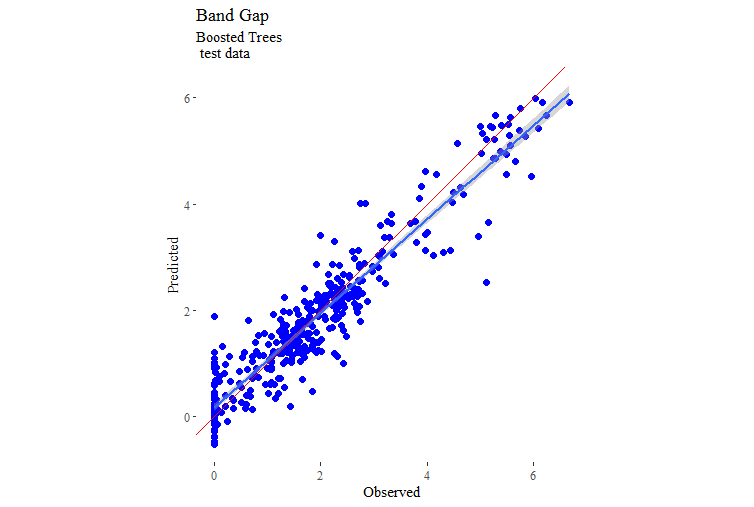
\includegraphics[scale = 0.375]{BoostedTreesTestDataFit.png}
\captionof{figure}{Boosted Trees: predicted vs observed. Adjusted \( R^2 = 0.8953 \)}.
\end{center}

\end{multicols}

\vspace*{1cm}
\begin{tabular*}{5.03\textwidth}{lr}
%\includegraphics[height=1.5cm,width=4cm]{signature_JY} & \includegraphics[height=1.5cm,width=4cm]{signature_F_clement} \\
Paul KOWALCZYK &\hspace*{9cm} Jean-Yves DELANNOY\\
\end{tabular*}

\tableofcontents

\chapter{Organization of this final report}

Four chapters follow:
\begin{description}
\item[Chapter 2. Introduction] This chapter introduces machine learning, describing both the construction of machine learning models and machine learning workflows.
\item[Chapter 3. Materials and Methods] This chapter describes
\begin{enumerate}
\item the data used in this study,
\item the features (descriptors) calculated for each compound, and
\item the machine learning algorithms employed.
\end{enumerate}
\item[Chapter 4. Results and Discussion] Each model built was evaluated with a set of test data. The results of each model's predictive performance on this test data is presented in this chapter. The selection of an optimal model is discussed.
\item[Chapter 5. Conclusion] The report concludes with a discussion of how this work may be generally applied.
\end{description}

\chapter{Introduction}

Machine learning models for materials properties are constructed from three parts
\begin{enumerate}
\item a training set,
\item a set of attributes describing each material, and
\item machine learning algorithms mapping the attributes to properties.
\end{enumerate}

\textsc{\textbf{A training set}}

Massive open-access databases of computed/predicted materials properties (including electronic structure, thermodynamic, and structural properties) are now available. [AFLOWLIB.ORG, Materials Project, Computational Materials Repository] Methods are sought to efficiently extract knowledge and mine trends out of these materials big-data repositories.

Given prior knowledge - in terms of high quality data on a given property of interest for a limited set of material candidates within a well defined chemical space - informatics based statistical learning approaches lead to efficient pathways to make high-fidelity predictions on new compounds within the target chemical space.

Our goal is the construction of validated statistical learning models for the prediction of bandgaps of sulfides. The models would establish a mathematical relationship (a \textit{mapping}) between the bandgap of material \textit{i} residing in the predefined chemical space, and an \(\Omega\)-dimensional (\(\Omega\)-D) feature vector f\textsubscript{\textit{i}} of the material \textit{i}.

\textsc{\textbf{A set of attributes describing each material}}

An attribute (also referred to as a feature; used interchangeably in this report) is an individual measurable property or characteristic of a object being studied. Choosing informative, discriminating and independent attributes is a crucial step for effective algorithms in pattern recognition, classification and regression.

The concept of "feature" is related to that of explanatory variable used in statistical techniques such as linear regression.

Features may be \textit{observed}, e.g., date of experiment, location of experiment, environmental conditions. Features may also be \textit{calculated}, e.g., molecular weight, number of atoms in a molecule, presence/absence of particular substructures.

The initial set of raw features can be redundant and too large to be managed. Therefore, a preliminary step in many applications of machine learning and pattern recognition consists of selecting a subset of features, or constructing a new and reduced set of features to facilitate learning, and to improve generalization and interpretability[citation needed].

Extracting or selecting features is a combination of art and science; developing systems to do so is known as feature engineering. It requires the experimentation of multiple possibilities and the combination of automated techniques with the intuition and knowledge of the domain expert. Automating this process is feature learning, where a machine not only uses features for learning, but learns the features itself.

Feature engineering is the process of using domain knowledge of the data to create features that make machine learning algorithms work.

\textsc{\textbf{Machine learning algorithms mapping the attributes to properties}}

Machine learning algorithms can be separated into two broad classes: \textit{supervised} and \textit{unsupervised} learning. In both of these classes, the algorithm has access to a set of observations known as \textit{training data}, the collection of known input (\textbf{X}) and output (\textsl{y}) values, which may be generated through observations or controlled experiments. The goal of the scientist is to use such training data, as well as any other prior knowledge, to identify a function that is able to predict the output value for a new set of input data accurately. In supervised learning, the training data consists of a set of \textit{input values} (e.g., the structures of different materials) as well as a corresponding set of \textit{output values} (e.g., materials property values). With these training data, the machine learning algorithm tries to identify a function that can make accurate predictions about the output values that will be associated with new input values. If the output values \textsl{y} form a continuous range (e.g., melting points), then the process of searching for a function is known as \textit{regression}. If the allowed output values form a discrete set (e.g., space groups), the process is then known as \textit{classification}. In unsupervised learning, there are no output values in the training data, and the goal is to identify patterns in the input values.


\textsc{Our approach to machine learning} is based on the \textbf{cr}oss-\textbf{i}ndustry \textbf{s}tandard \textbf{p}rocess for \textbf{d}ata \textbf{m}ining (CRISP-DM). A process diagram of this process is presented in Figure 2.1.

\begin{center}
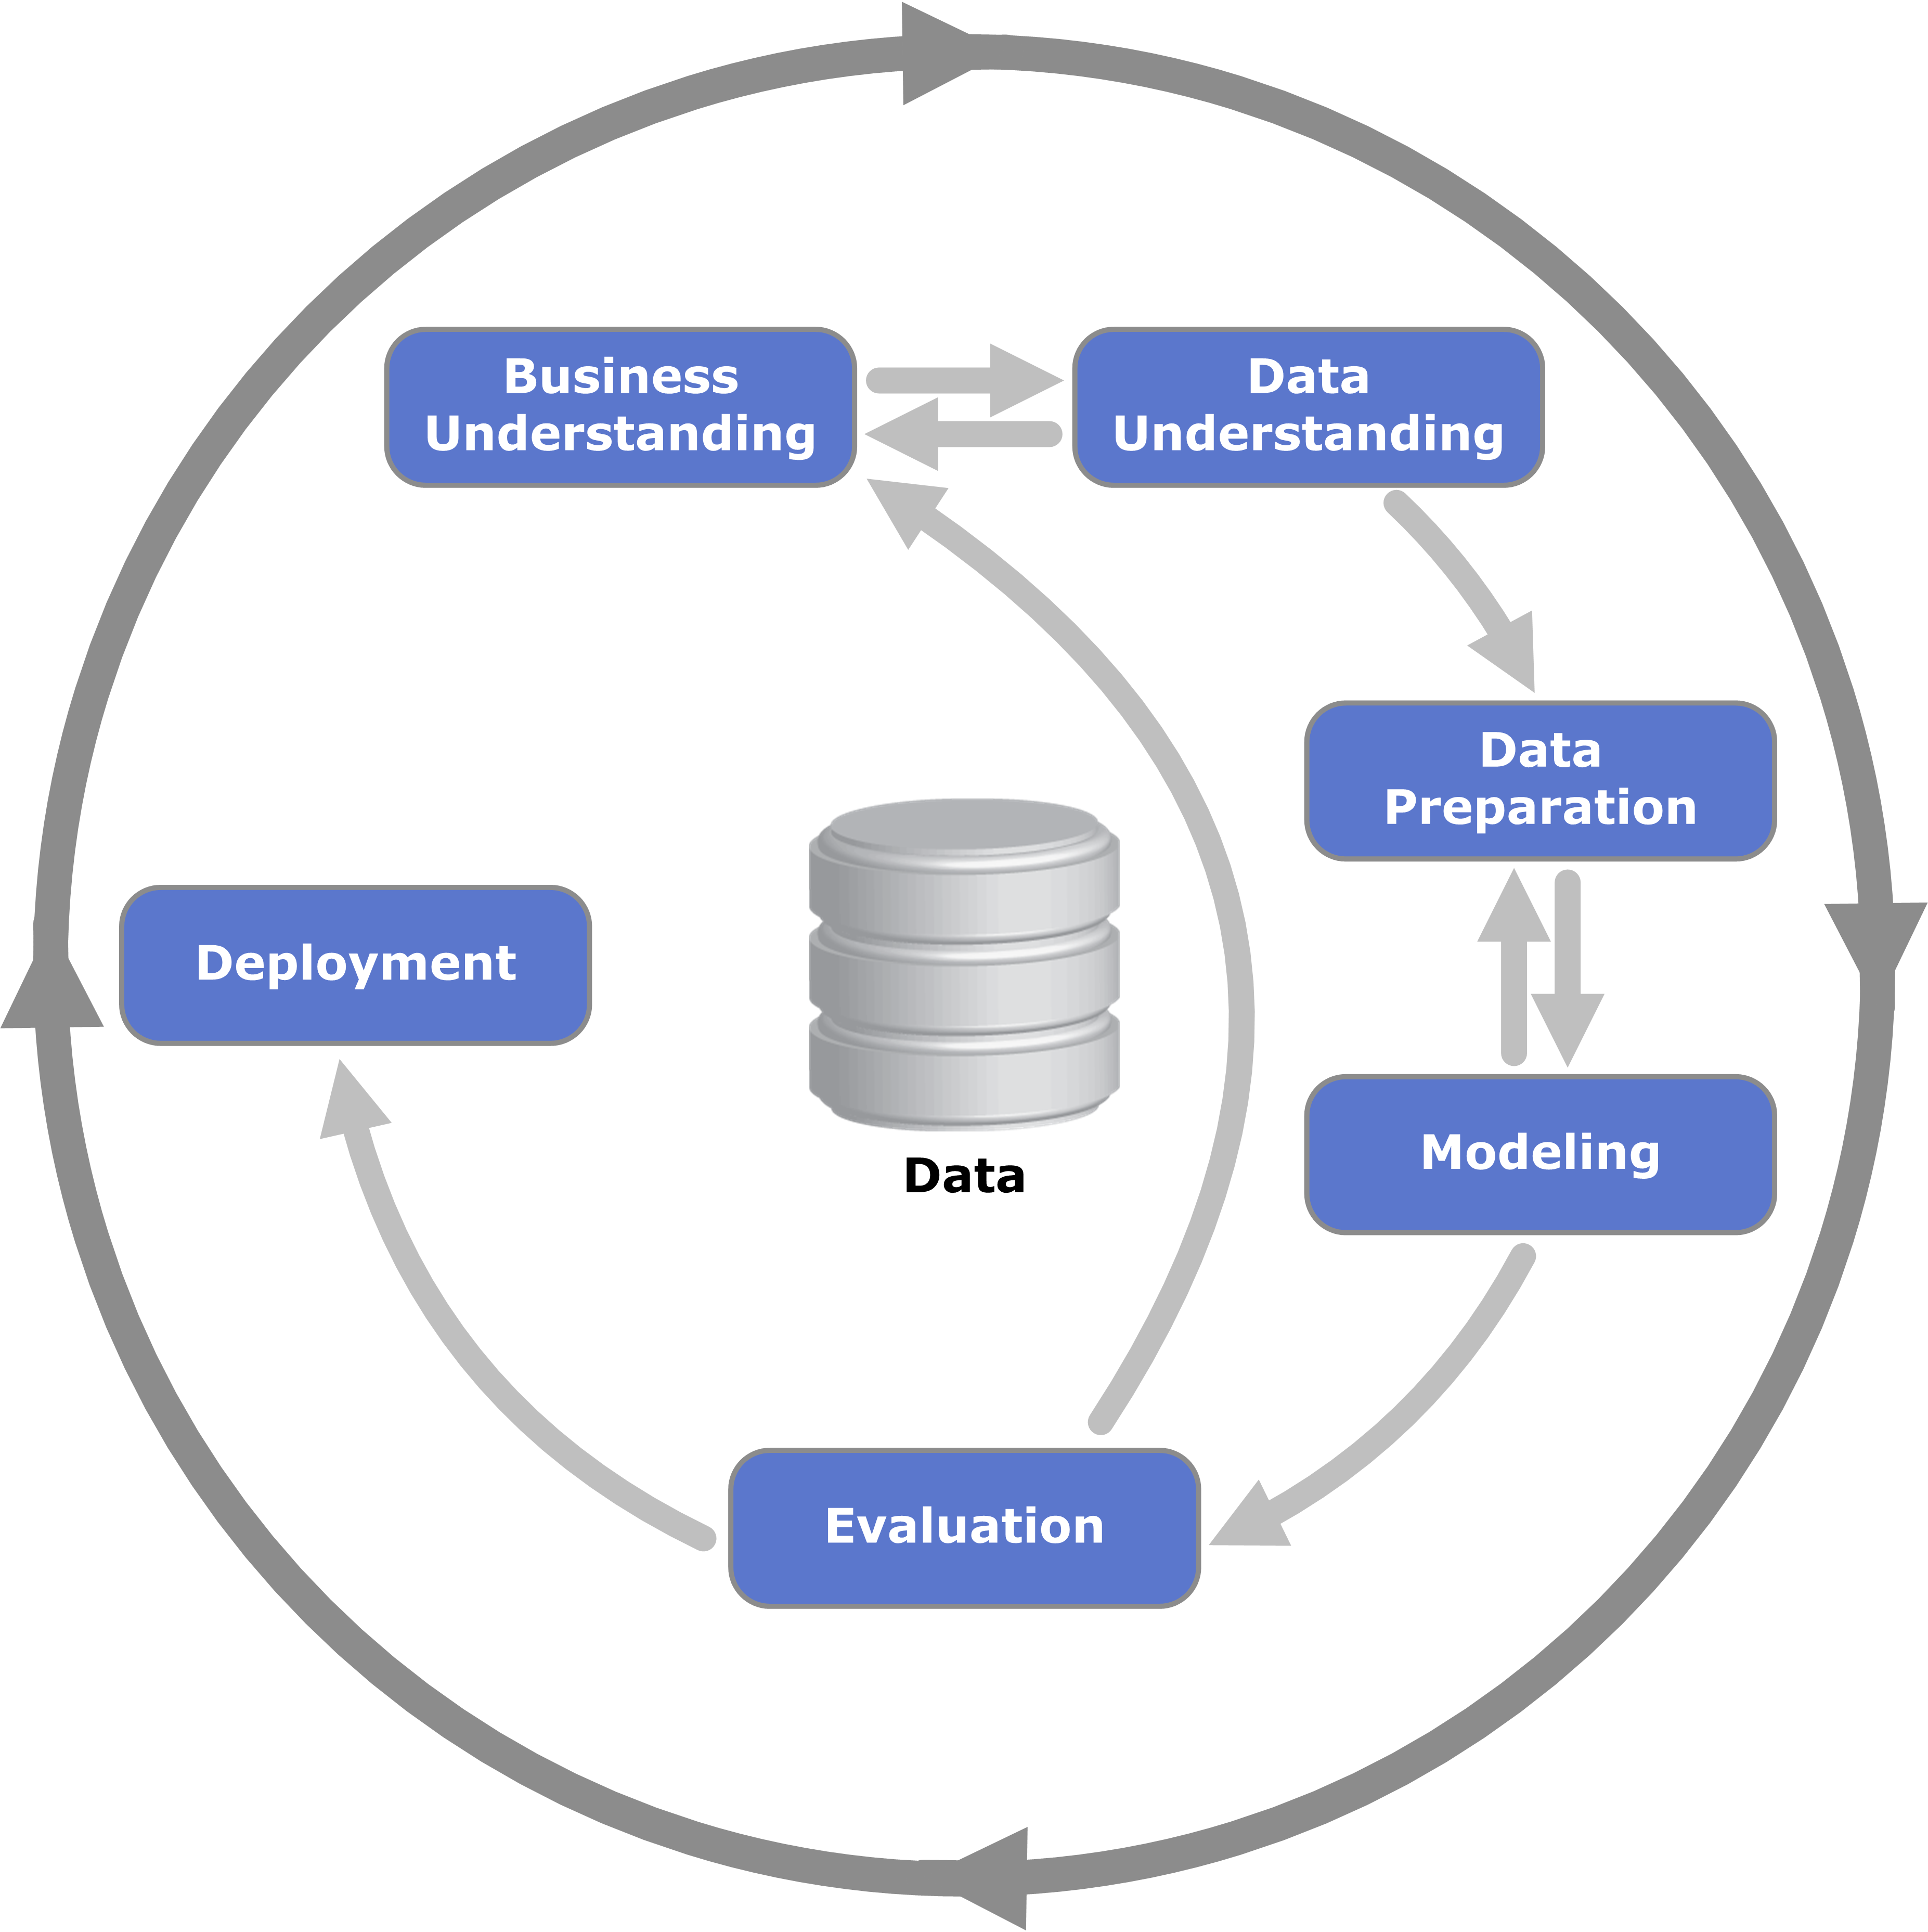
\includegraphics[scale=0.35]{CRISP-DM_Process_Diagram.png}
\captionof{figure}{Process diagram of the CRISP-DM process.}
\end{center}

CRISP-DM breaks the process of data mining into six major phases. The sequence of the phases is not strict, and moving back and forth between different phases is always required. The arrows in the process diagram indicate the most important and frequent dependencies between phases. The outer circle in the diagram symbolizes the cyclic nature of data mining itself. A data mining process continues after a solution has been deployed. The lessons learned during the process can trigger new, often more focused business questions, and subsequent data mining processes will benefit from the experiences of previous ones.

During the \textbf{business understanding} phase business objectives and requirements are investigated; decisions are made as to whether data mining can be applied to meet them; and determinations are made regarding the data that can be collected to build a deployable model. During the \textbf{data understanding} phase an initial dataset is established and studied to see whether it is suitable for further processing. Insights gained during this stage may lead to collecting new data or, in some cases, reconsidering the utility of a data mining campaign.

An actual example of \textbf{data preparation}, \textbf{modeling}, and \textbf{evaluation} is presented throughout this report. Preparation involves preprocessing the raw data so that machine learning algorithms can produce a model. During the modeling phase numerous algorithms are used to construct relationships between the features (\textbf{X}) and outcomes (\textsl{y}). The importance of the \textbf{evaluation} phase cannot be overstated. Only those models showing high accuracy and predictive ability merit further consideration. It can happen that no acceptable model is identified.

One enters the \textbf{deployment} phase once an acceptable model has been identified. Here, the model is democratized, i.e., made generally available. Discussions of model deployment are outside the scope of this report.

\chapter{Materials and Methods}

\section{Data Set}
\textsc{Data for this report} were retrieved from the Materials Project. Nine properties were retrieved for each entry:
\begin{description}
\item[pretty\_formula] a nice formula where the element amounts are normalized
\item[unit\_cell\_formula] the full explicit formula for the unit cell
\item[energy] calculated VASP energy for structure (the Vienna Ab-initio Simulation Package (VASP) is a software package that uses density functional theory to solve the quantum problem for materials)
\item[band\_gap] the calculated band gap
\item[e\_above\_hull] calculated energy above convex hull for structure
\item[nelements] the number of elements in the material
\item[spacegroup.crystal\_system] the crystal system for the space group
\item[spacegroup.number] the number for the space group
\item[spacegroup.symbol] the symbol for the space group
\end{description}

A total of 83989 entries were retrieved.

Only energetically stable compounds were considered in this workflow. Consequently, only those compounds with e\_above\_hull \(\leq 10^{-9}\) were retained. 25370 entries had an e\_above\_hull \(\leq 10^{-9}\).

Further, only sulfides were considered in this workflow. There were 1989 sulfides amongst the 25370 stable compounds.

A sampling of the retrieved data is presented in Table 3.1.


\begin{table}[H]
\begin{center}
\begin{tabular}{rrr}
\toprule
% \hline
&&\\
{\bf composition} & {\bf band gap} & {\bf unit cell formula}\\
% &&\\
%\hline
\midrule
&&\\
BaCdGeS4  &   2.7009 & {'S': 32.0, 'Ge': 8.0, 'Cd': 8.0, 'Ba': 8.0} \\
AgBiSCl2 &  1.0687  & {'Ag': 2.0, 'Bi': 2.0, 'S': 2.0, 'Cl': 4.0} \\
NbCu3S4  & 1.6574     &        {'Nb': 1.0, 'Cu': 3.0, 'S': 4.0} \\
K2NdP2S7 &  2.3533  & {'P': 8.0, 'S': 28.0, 'K': 8.0, 'Nd': 4.0} \\ 
Cu3SbS4 &  0.0000    &         {'S': 4.0, 'Cu': 3.0, 'Sb': 1.0} \\
BaCu2SnS4 &  0.3869 & {'S': 12.0, 'Cu': 6.0, 'Sn': 3.0, 'Ba': 3.0} \\
KSb(PS3)2 &  2.2673   & {'K': 2.0, 'Sb': 2.0, 'P': 4.0, 'S': 12.0} \\
ThAsS &  0.0000         &    {'Th': 2.0, 'As': 2.0, 'S': 2.0} \\
K3Cu2(BiS2)5 &  0.5758 & {'K': 6.0, 'Cu': 4.0, 'Bi': 10.0, 'S': 20.0} \\
MgSO4 &  5.4889          &    {'O': 8.0, 'Mg': 2.0, 'S': 2.0} \\
&&\\
%\hline
\bottomrule
\end{tabular}
\end{center}
\caption{Sampling of data retrieved from the Materials Project.}
\end{table}

\section{Features}
Features were calculated using Magpie [\textbf{M}aterials-\textbf{Ag}nostic \textbf{P}latform for \textbf{I}nformatics and \textbf{E}xploration] (REFERENCE\: A general\-purpose machine learning framework for predicting properties of inorganic materials. Logan Ward, Ankit Agrawal, Alok Choudhary \& Christopher Wolverton. npj Computational Materials volume 2, Article number\: 16028 (2016)).

Magpie allows for the calculation of an expansive set of attributes that can be used for materials with any number of constituent elements. This set is broad enough to capture a sufficiently diverse range of physical/chemical properties to be used to create accurate models for many materials problems. In total, a set of 145 attributes are calculated. These attributes fall into four distinct categories:
\begin{enumerate}
\item \textbf{Stoichiometric attributes} that depend only on the fractions of elements present and not what those elements actually are. These include the number of elements present in the compound and several Lp norms of the fractions.
\item \textbf{Elemental property statistics}, which are defined as the mean, mean absolute deviation, range, minimum, maximum and mode of 22 different elemental properties. This category includes attributes such as the maximum row on periodic table, average atomic number and the range of atomic radii between all elements present in the material.
\item \textbf{Electronic structure attributes}, which are the average fraction of electrons from the s, p, d and f valence shells between all present elements.
\item \textbf{Ionic compound attributes} that include whether it is possible to form an ionic compound assuming all elements are present in a single oxidation state, and two adaptations of the fractional ‘ionic character’ of a compound based on an electronegativity-based measure.
\end{enumerate}

\section{Classifiers}

\chapter{Results and Discussion}

\section{Building the training set and the test set}
\begin{center}
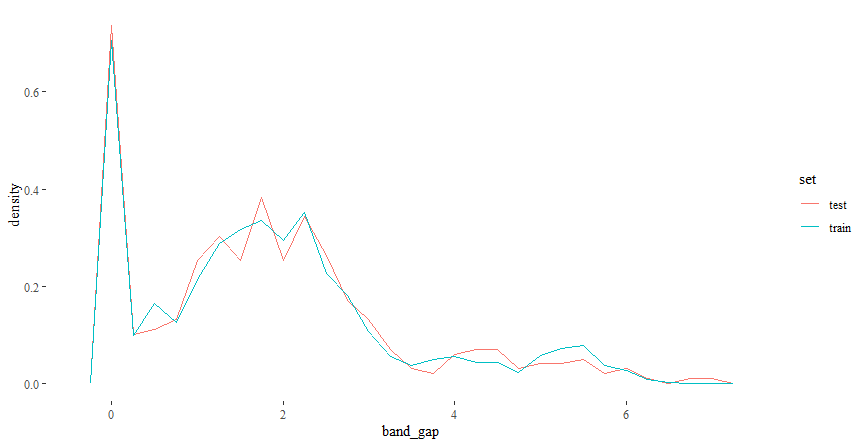
\includegraphics[scale=0.35]{train_test_distributions.png}
\captionof{figure}{Density distributions for bandgap energies in the training and test sets.}
\end{center}

\section{Feature Engineering}
\subsection{Zero variance features}
Seven of the calculated features for the training set have zero variance (i.e., are single-valued). These features are max\_NsValence, min\_NdValence, min\_NfValence, min\_NsUnfilled, min\_NdUnfilled, and min\_NfUnfilled, min\_GSmagmom. These features are removed from both the training set and the test set.

\subsection{Feature Correlation}
\begin{center}
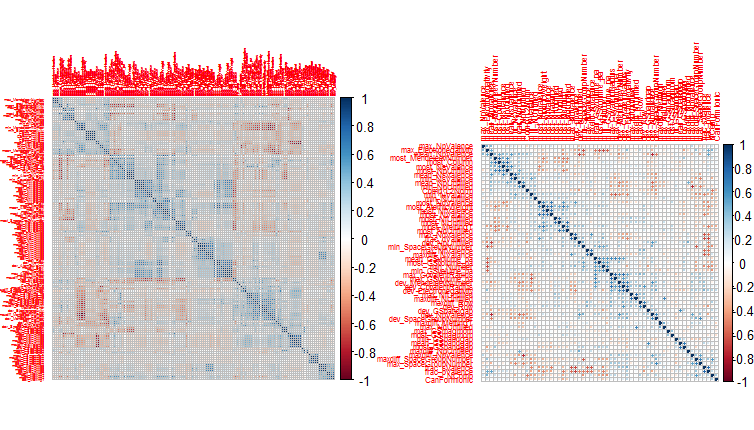
\includegraphics[scale = 0.8]{CorrelatedFeatures.png}
\captionof{figure}{Graphical display of the feature correlation matrix before (left) and after (right) removing highly correlated features.}
\end{center}

\section{Machine Learning Models}

\subsection{Multiple Linear Regression}

\begin{center}
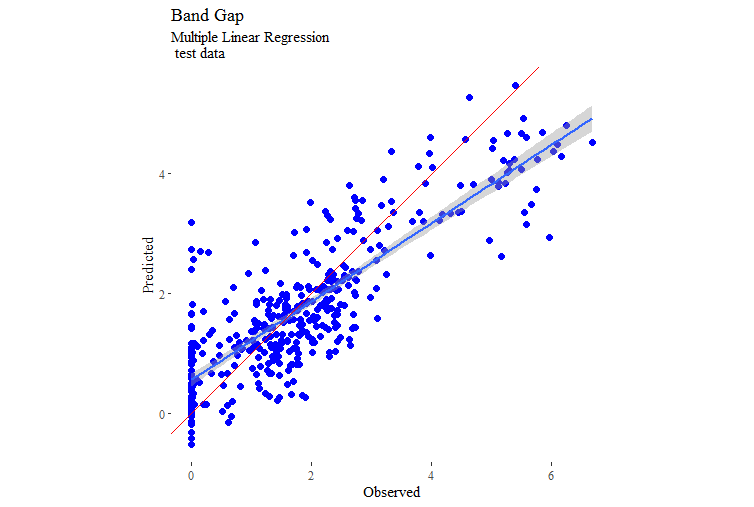
\includegraphics[scale = 0.8]{MLRTestDataFit.png}
\captionof{figure}{Multiple Linear Regression: predicted vs observed. Adjusted \( R^2 = 0.6947 \)}
\end{center}

\subsection{Partial Least Squares}

\begin{center}
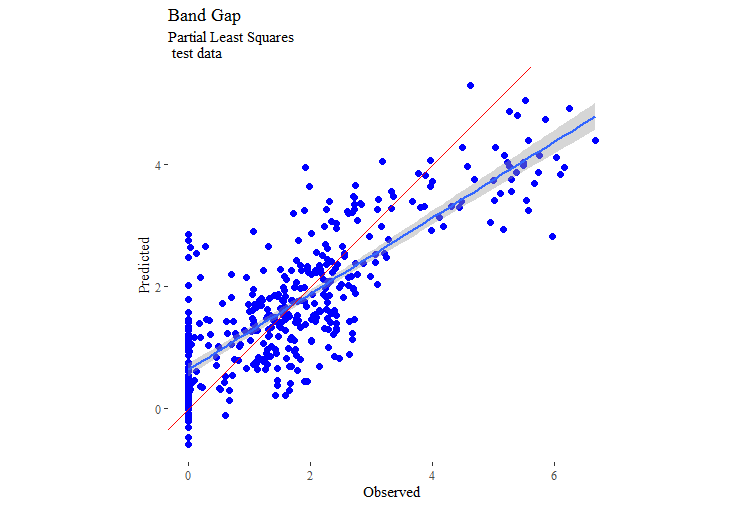
\includegraphics[scale = 0.8]{PLSTestDataFit.png}
\captionof{figure}{Partial Least Squares: predicted vs observed. Adjusted \( R^2 = 0.6652 \)}
\end{center}

\subsection{Support Vector Machine}

\begin{center}
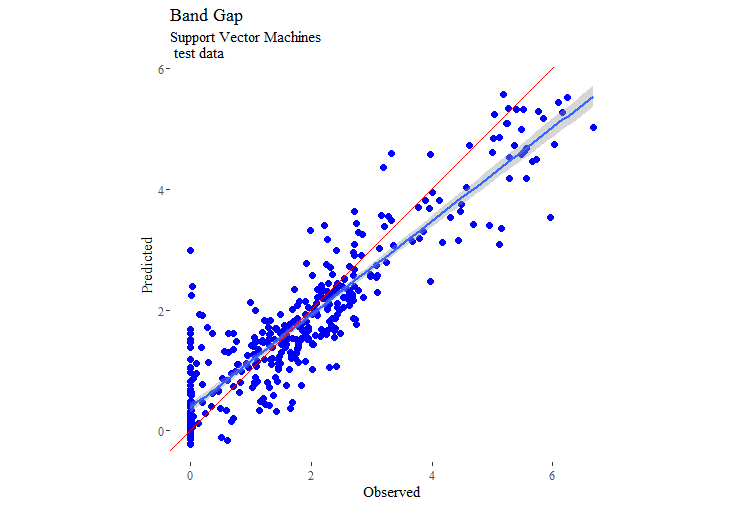
\includegraphics[scale = 0.8]{SVMTestDataFit.png}
\captionof{figure}{Support Vector Machine: predicted vs observed. Adjusted \( R^2 = 0.8294 \)}
\end{center}

\subsection{K-Nearest Neighbors}

\begin{center}
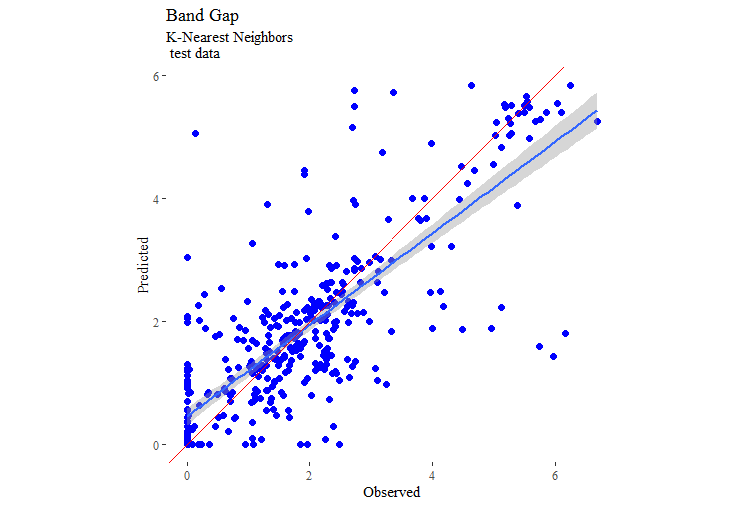
\includegraphics[scale = 0.8]{KNNTestDataFit.png}
\captionof{figure}{K-Nearest Neighbors: predicted vs observed. Adjusted \( R^2 = 0.6207 \)}
\end{center}

\subsection{Random Forest}

\begin{center}
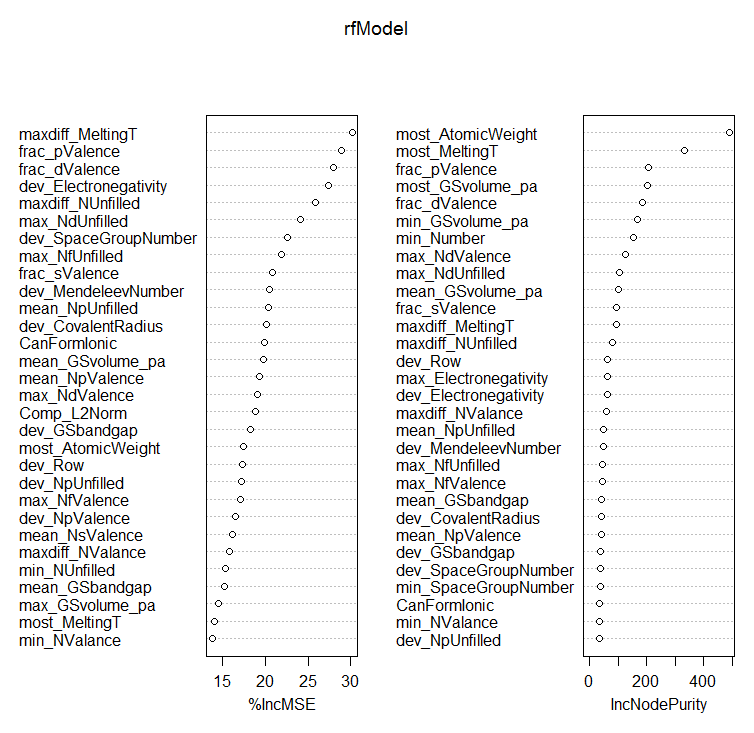
\includegraphics[scale = 0.8]{RandomForestVariableImportance.png}
\captionof{figure}{Random Forest: variable importance plots.}
\end{center}

\begin{center}
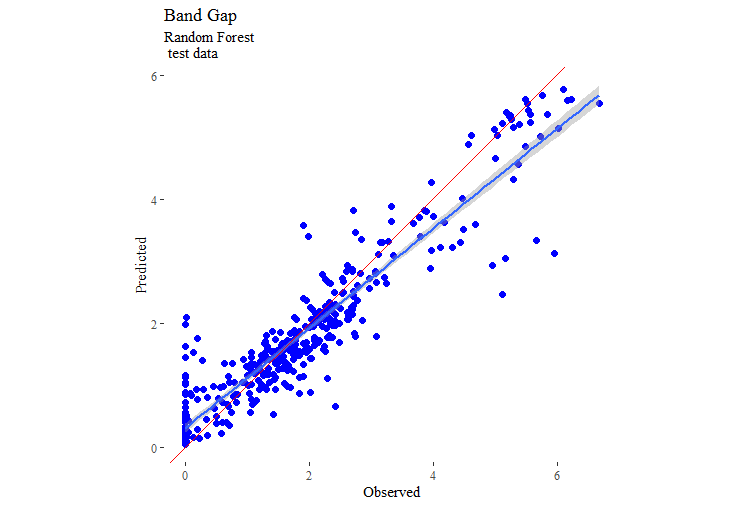
\includegraphics[scale = 0.8]{RandomForestTestDataFit.png}
\captionof{figure}{Random Forest: predicted vs observed. Adjusted \( R^2 = 0.8746 \)}.
\end{center}

\subsection{Boosted Trees}

\begin{center}
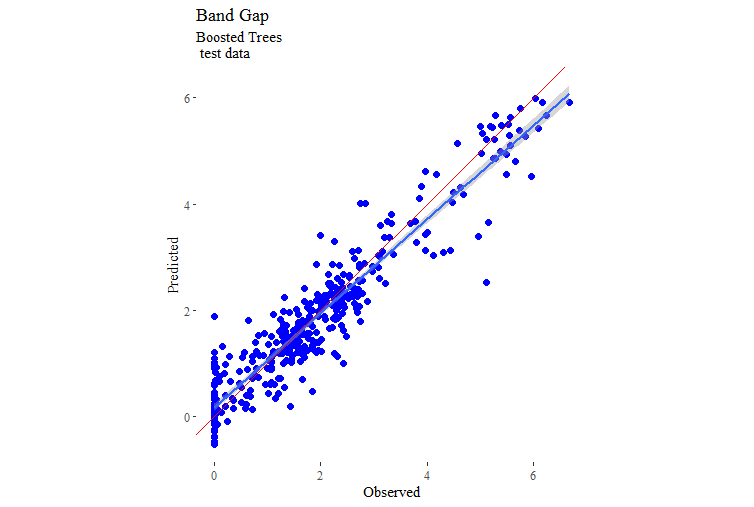
\includegraphics[scale = 0.8]{BoostedTreesTestDataFit.png}
\captionof{figure}{Boosted Trees: predicted vs observed. Adjusted \( R^2 = 0.8953 \)}.
\end{center}

\chapter{Conclusion}

\begin{table}[H]
\begin{center}
\begin{tabular}{rrr}
\toprule
% \hline
&&\\
{\bf Machine Learning Method} & {\bf Adjusted \( R^2 \)} \\
% &&\\
%\hline
\midrule
&&\\
Multiple Linear Regression  &   0.6947 \\
Partial Least Squares &  0.6652 \\
Support Vector Machine  & 0.8294 \\
K-Nearest Neighbors &  0.6207 \\ 
Boosted Trees &  0.8953 \\
Random Forest &  0.8746 \\
&&\\
%\hline
\bottomrule
\end{tabular}
\end{center}
\caption{Summary of machine learning experiments.}
\end{table}

\newpage
\begin{center}
{\bf FICHE RESUME/BIBLIOGRAPHICAL FORM DOCUMENTUM}
\end{center}
\begin{flushleft}
\begin{tabular}{|l|p{0.18\textwidth}|p{0.63\textwidth}|}
\hline
&&\\
{\bf SERVICE} & Laboratory Group & SM@RT\\
&&\\ \hline &&\\
{\bf Type de document} & Document type & Rapport de Projet \\
&&\\ \hline &&\\
\bf Date & Application Date & Decembre 2014\\
&&\\ \hline &&\\
{\bf TITRE en Anglais} & English Title & COMPNANOCOMP FP7 Project : Final Report \\
&&\\ \hline &&\\
{\bf TITRE en Français} & French Title & Projet FP7 COMPNANOCOMP : Rapport Final \\
&&\\ \hline &&\\
\bf Entreprise & Enterprises/Sponsors & R$\&$I/AIO/Advanced Materials Platform  \\
&&\\ \hline &&\\
\bf Auteur(s) & Authors & Jean Yves DELANNOY \\
&&\\ \hline &&\\
\bf PROJET & Projects & COMPNANOCOMP\\
&&\\ \hline &&\\
\bf Collaborateurs & Collaborators & Cédric Feral-Martin\\
&& Aur\'elie Papon\\
&& Magali Fontana\\
&& Olivier Sanseau \\
&&\\ \hline &&\\
\bf N$^0$ d'affaire & Business code & \\
&&\\ \hline &&\\

\bf RESUME  Anglais & & The objective of this document is to offer a "digest" of the main results obtained  in this project that aims at the development of multiscale simulation methodology and software for predicting the morphology (spatial distribution and state of aggregation of nanoparticles), thermal (glass temperature), mechanical (viscoelastic storage and loss moduli, plasticity, fracture toughness and compression strength), electrical and optical properties of soft and hard polymer matrix nanocomposites from the atomic-level characteristics of their constituent nanoparticles and macromolecules and from the processing conditions used in their preparation.

The document gives a short summary of the results obtained within this project by Solvay and its partners. It also emphasizes the interest for Solvay R$\&$I of  the developments obtained. 


\\
&&\\ 
\hline
\end{tabular}

\begin{tabular}{|l|p{0.18\textwidth}|p{0.63\textwidth}|}
\hline
&&\\
\bf RESUME Français &&  L'objectif de ce rapport est de fournir un résumé des points essentiels développés dans le rapport final du projet européen FP7 COMPNANOCOMP dont le but est de développer une méthodologie de simulation multi-échelle permettant de prédire la morphologie (distribution spatiale et état d'agrégation des nanoparticules), et les propriétés thermiques, mécaniques optiques et électriques de nanocomposites de polymères. Ce travail s'effectue sur la base des caractéristiques atomiques des constituants du matériaux et doit prendre en compte les conditions du procédé ayant permis sa réalisation.

Ce document donne une vision des résultats obtenus par Solvay et ses collaborateurs et met en avant l'intérêt pour le groupe des développements effectués.
\\
&&\\ \hline &&\\
\bf Mots Clés Anglais & English Keywords&  RUBBER, REINFORCEMENT, SILICA, COUPLING, MODELING, MORPHOLOGY, FP7\\
&&\\ \hline &&\\
\bf Mots Clés Français &&  CAOUTCHOUC ; RENFORT ; SILICE ; COUPLAGE ; MODELISATION ; MORPHOLOGIE, FP7\\
&&\\ \hline &&\\
\bf RNCAS & RNCAS & \\
&&\\ \hline &&\\
\bf Destinataires& Addressees & \\
&&\\ \hline &&\\
\bf CONFIDENTIEL & Confidential & YES \\
&&\\ \hline
\end{tabular}



\end{flushleft}




\end{document}





